%\begin{figure}
%\begin{tikzpicture}[arrow/.style={line width=1pt,->,>=latex}]
%	\draw [line width=1pt] (-2,1) rectangle (2,-1) node at (0,0) {$j$};
%	\draw [arrow] (-1,3) -- (-1,1) node [pos=0.25, left] {\footnotesize $L_{j-1}$};
% 	\draw [arrow] (-3.5,1.7) -- (-1,1.7) node [pos=0.25, above] {\footnotesize $F^L_{j}$};
% 	\draw [arrow] (1,1) -- (1,3) node [pos=0.75, right] {\footnotesize $V_{j}$};
% 	\draw [arrow] (1,1.7) -- (3.5,1.7) node [pos=0.75, above] {\footnotesize $S^V_{j}$};
% 	\draw [arrow] (-1,-1) -- (-1,-3) node [pos=0.75, left] {\footnotesize $L_{j}$};
% 	\draw [arrow] (-1,-1.7) -- (-3.5,-1.7) node [pos=0.75, above] {\footnotesize $S^L_{j}$};
%	\draw [arrow] (1,-3) -- (1,-1) node [pos=0.25, right] {\footnotesize $V_{j+1}$};
%	\draw [arrow] (3.5,-1.7) -- (1,-1.7) node [pos=0.25, above] {\footnotesize $F^V_{j}$};
%	\draw [arrow] (2,0) -- (3,0) -- (3.2,0.5) -- (3.4,-0.5) -- (3.6,0.5) -- (3.8,-0.5) -- (3.9,0) -- (5,0,0) node [pos=1, right] {\footnotesize $Q$} ;
%    \draw [line width=0.5pt,gray] (-2,-3.5) -- (-2,-3) -- (2,-3) node [pos=0.5, below] {$j+1$} -- (2,-3.5) ;
%    \draw [line width=0.5pt,gray] (-2,3.5) -- (-2,3) -- (2,3) node [pos=0.5, above] {$j-1$} -- (2,3.5) ;
%\end{tikzpicture}
%\end{figure}
%
%% complete column superstructure
%\begin{figure}
%\begin{tikzpicture}[arrow/.style={line width=1pt,->,>=latex},scale=0.7]
%	\draw [line width=0.5pt,gray] (1,4.8) -- (-1,4.8) node [above,pos=0.5,black] {\scriptsize 1};
%    \draw [line width=0.5pt,gray] (1,-4.8) -- (-1,-4.8) node [above,pos=0.5,black] {\scriptsize N};
%    \draw [line width=0.5pt,gray] (1,-4.0) -- (-1,-4.0) node [above,pos=0.5,black] {};
%    \draw [line width=0.5pt,gray] (1,-3.2) -- (-1,-3.2) node [above,pos=0.5,black] {};
%    \draw [line width=0.5pt,gray] (1,-0.8) -- (-1,-0.8) node [above,pos=0.5,black] {};
%    \draw [line width=0.5pt,gray] (1,0.0) -- (-1,0.0) node [above,pos=0.5,black] {};
%    \draw [line width=0.5pt,gray] (1,0.8) -- (-1,0.8) node [above,pos=0.5,black] {};
%    \draw [line width=0.5pt,gray] (1,1.6) -- (-1,1.6) node [above,pos=0.5,black] {};
%    %\draw [line width=0.5pt,gray] (1,2.4) -- (-1,2.4) node [above,pos=0.5,black] {};
%	\draw [line width=1pt, rounded corners] (-1.0,-5) -- (-1.0,5) .. controls (-0.8,5.8) and (0.8,5.8) .. (1.0,5) node (a) [inner sep=0cm , pos=0.5] {} -- (1.0,-5) .. controls (0.8,-5.8) and (-0.8,-5.8) .. (-1.0,-5) node (b) [inner sep=0cm , pos=0.5] {} -- cycle ; % column tower
%    \draw [arrow] (2.5,6.2) -- (2.5,7.5) -- (4.0,7.5) ;
%	\draw [arrow] (a) -- (0,6.2) -- (2.5,6.2) node [draw, thick, pos=1, circle, minimum size=1.2cm, fill=white] {} -- (2.5,4.8) -- (1,4.8) ;   % circle condenser
%    \draw [arrow] (b) -- (0,-6.2) -- (2.5,-6.2) node [draw, thick, pos=1, circle, minimum size=1.2cm, fill=white] {} -- (2.5,-4.8) -- (1,-4.8) ; % circle reboiler
%	\draw [line width=0.5pt] (4,6.5) -- (2.2,6.5) -- (2.6,6.2) -- (2.2,5.9) -- (4,5.9) ;   % heater condenser
%    \draw [line width=0.5pt] (4,-6.5) -- (2.2,-6.5) -- (2.6,-6.2) -- (2.2,-5.9) -- (4,-5.9) ; % heater reboiler
%	\draw [arrow] (2.5,4.8) -- (4,4.8) ;
%    \draw [arrow] (2.5,-4.8) -- (4,-4.8) ;
%    \draw [arrow] (2.0,-4.8) -- (2.0,-4.0) -- (1.0,-4.0) ;
%    \draw [arrow] (2.0,-4.0) -- (2.0,-3.2) -- (1.0,-3.2) ;
%    \draw [arrow] (-3.0,0.8) -- (-1.0,0.8) ;
%    \draw [arrow] (-2.0,0.8) -- (-2.0,1.6) -- (-1.0,1.6) ;
%    %\draw [arrow] (-2.0,1.6) -- (-2.0,2.4) -- (-1.0,2.4) ;
%    \draw [arrow] (-2.0,0.8) -- (-2.0,0.0) -- (-1.0,0.0) ;
%    \draw [arrow] (-2.0,0.0) -- (-2.0,-0.8) -- (-1.0,-0.8) ;
%    \node (C) [draw, line width=0.5pt, circle, gray, minimum size=1.6cm] at (0,0.8){} ;
%    \node (D) [draw, line width=0.5pt, circle, gray, minimum size=8cm] at (13,0) {} ;
%    	\draw [line width=1pt] (10,1) rectangle (14,-1) node at (12,0) {$j$};
%	\draw [arrow] (11,3) -- (11,1) node [pos=0.25, left] {\footnotesize $L_{j-1}$};
% 	\draw [arrow] (8.5,1.7) -- (11,1.7) node [pos=0.25, above] {\footnotesize $F^L_{j}$};
% 	\draw [arrow] (13,1) -- (13,3) node [pos=0.75, right] {\footnotesize $V_{j}$};
% 	\draw [arrow] (13,1.7) -- (15.5,1.7) node [pos=0.75, above] {\footnotesize $S^V_{j}$};
% 	\draw [arrow] (11,-1) -- (11,-3) node [pos=0.75, left] {\footnotesize $L_{j}$};
% 	\draw [arrow] (11,-1.7) -- (8.5,-1.7) node [pos=0.75, above] {\footnotesize $S^L_{j}$};
%	\draw [arrow] (13,-3) -- (13,-1) node [pos=0.25, right] {\footnotesize $V_{j+1}$};
%	\draw [arrow] (15.5,-1.7) -- (13,-1.7) node [pos=0.25, above] {\footnotesize $F^V_{j}$};
%	\draw [arrow] (14,0) -- (15,0) -- (15.2,0.5) -- (15.4,-0.5) -- (15.6,0.5) -- (15.8,-0.5) -- (15.9,0) -- (17,0,0) node [pos=1, right] {\footnotesize $Q$} ;
%    \draw [line width=0.5pt,gray] (10,-3.5) -- (10,-3) -- (14,-3) node [pos=0.5, below] {$j+1$} -- (14,-3.5) ;
%    \draw [line width=0.5pt,gray] (10,3.5) -- (10,3) -- (14,3) node [pos=0.5, above] {$j-1$} -- (14,3.5) ;
%    %\draw [line width=0.5pt,gray] (C.north) -- (D.north) ;
%\end{tikzpicture}
%\end{figure}

\begin{figure}
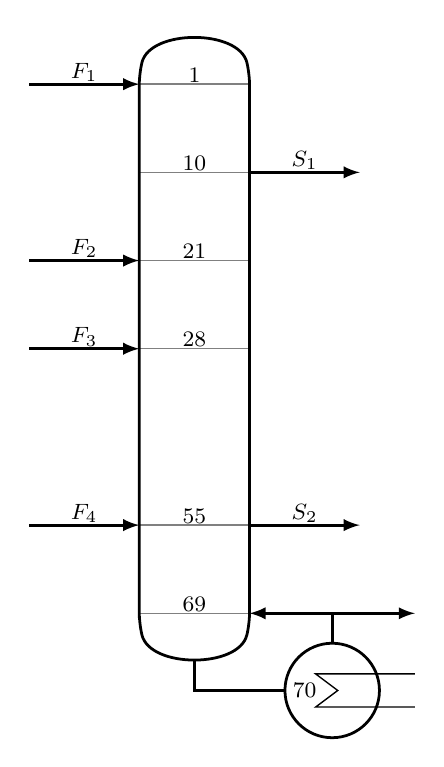
\begin{tikzpicture}[arrow/.style={line width=1pt,->,>=latex},scale=0.7]
	\draw [line width=0.5pt,gray] (1,4.8) -- (-1,4.8) node [above,pos=0.5,black,yshift=-1mm] {\footnotesize 1};
    \draw [line width=0.5pt,gray] (1,-4.8) -- (-1,-4.8) node [above,pos=0.5,black,yshift=-1mm] {\footnotesize 69};
    \draw [line width=0.5pt,gray] (1,3.2) -- (-1,3.2) node [above,pos=0.5,black,yshift=-1mm] {\footnotesize 10};
    \draw [line width=0.5pt,gray] (1,1.6) -- (-1,1.6) node [above,pos=0.5,black,yshift=-1mm] {\footnotesize 21};
    \draw [line width=0.5pt,gray] (1,0.0) -- (-1,0.0) node [above,pos=0.5,black,yshift=-1mm] {\footnotesize 28};
    \draw [line width=0.5pt,gray] (1,-3.2) -- (-1,-3.2) node [above,pos=0.5,black,yshift=-1mm] {\footnotesize 55};
	\draw [line width=1pt, rounded corners] (-1.0,-5) -- (-1.0,5) .. controls (-0.8,5.8) and (0.8,5.8) .. (1.0,5) node (a) [inner sep=0cm , pos=0.5] {} -- (1.0,-5) .. controls (0.8,-5.8) and (-0.8,-5.8) .. (-1.0,-5) node (b) [inner sep=0cm , pos=0.5] {} -- cycle ; % column tower
    \draw [arrow] (b) -- (0,-6.2) -- (2.5,-6.2) node [draw, line width=1pt, pos=1, circle, minimum size=1.2cm, fill=white] {} -- (2.5,-4.8) -- (1,-4.8) ; % circle reboiler
    \draw [line width=0.5pt] (4,-6.5) -- (2.2,-6.5) -- (2.6,-6.2) -- (2.2,-5.9) -- (4,-5.9) ; % heater reboiler
	\draw [arrow] (-3.0,4.8) -- (-1,4.8) node [above,pos=0.5,black,yshift=-1mm] {\footnotesize $F_1$} ;
    \draw [arrow] (-3.0,1.6) -- (-1,1.6) node [above,pos=0.5,black,yshift=-1mm] {\footnotesize $F_2$} ;
    \draw [arrow] (-3.0,0.0) -- (-1,0.0) node [above,pos=0.5,black,yshift=-1mm] {\footnotesize $F_3$} ;
    \draw [arrow] (-3.0,-3.2) -- (-1,-3.2) node [above,pos=0.5,black,yshift=-1mm] {\footnotesize $F_4$} ;
    \draw [arrow] (1.0,3.2) -- (3.0,3.2) node [above,pos=0.5,black,yshift=-1mm] {\footnotesize $S_1$} ;
    \draw [arrow] (1.0,-3.2) -- (3,-3.2) node [above,pos=0.5,black,yshift=-1mm] {\footnotesize $S_2$} ;
    \draw [arrow] (2.5,-4.8) -- (4,-4.8) ;
    \node at (2.0,-6.2) {\footnotesize 70} ;
\end{tikzpicture}
\end{figure}

\stdfig{pgfplots/LPC_O2_INIT}{O2 Init}{fig:O2:Init}{}

%\begin{figure}
%\begin{tikzpicture}[arrow/.style={line width=1pt,->,>=latex},scale=0.7]
%    \draw [line width=0.5pt,gray] (1,4.8) -- (-1,4.8) node [above,pos=0.5,black] {\scriptsize 1};
%    \draw [line width=0.5pt,gray] (1,-4.8) -- (-1,-4.8) node [above,pos=0.5,black] {\scriptsize N};
%    \draw [line width=0.5pt,gray] (1,-4.0) -- (-1,-4.0) node [above,pos=0.5,black] {};
%    \draw [line width=0.5pt,gray] (1,-3.2) -- (-1,-3.2) node [above,pos=0.5,black] {};
%    \draw [line width=0.5pt,gray] (1,-0.8) -- (-1,-0.8) node [above,pos=0.5,black] {};
%    \draw [line width=0.5pt,gray] (1,0.0) -- (-1,0.0) node [above,pos=0.5,black] {};
%    \draw [line width=0.5pt,gray] (1,0.8) -- (-1,0.8) node [above,pos=0.5,black] {};
%    \draw [line width=0.5pt,gray] (1,1.6) -- (-1,1.6) node [above,pos=0.5,black] {};
%    \draw [line width=1pt, rounded corners] (-1.0,2.8) -- (-1.0,5) .. controls (-0.8,5.8) and (0.8,5.8) .. (1.0,5) node (a) [inner sep=0cm , pos=0.5] {} -- (1.0,2.8);
%    \draw [arrow] (a) -- (0,6.2) -- (2.5,6.2) node [draw, thick, pos=1, circle, minimum size=1.2cm, fill=white] {} -- (2.5,4.8) -- (1,4.8) ; % condenser
%    \draw [line width=0.5pt] (4,6.5) -- (2.2,6.5) -- (2.6,6.2) -- (2.2,5.9) -- (4,5.9) ;   % heater condenser
%    \draw [line width=1pt] (1.0,2.6) .. controls (0.75,2.85) and (0.25,2.85) .. (0.0,2.6) .. controls (-0.25,2.35) and (-0.75,2.35) .. (-1.0,2.6);
%    \draw [line width=1pt] (1.0,-2.2) .. controls (0.75,-2.45) and (0.25,-2.45) .. (0.0,-2.2) .. controls (-0.25,-1.95) and (-0.75,-1.95) .. (-1.0,-2.2);
%    \draw [line width=1pt] (1.0,2.8) .. controls (0.75,3.05) and (0.25,3.05) .. (0.0,2.8) .. controls (-0.25,2.55) and (-0.75,2.55) .. (-1.0,2.8);
%    \draw [line width=1pt] (1.0,-2.4) .. controls (0.75,-2.65) and (0.25,-2.65) .. (0.0,-2.4) .. controls (-0.25,-2.15) and (-0.75,-2.15) .. (-1.0,-2.4);
%    \draw [line width=1pt] (1.0,2.6) -- (1.0,-2.2) ;
%    \draw [line width=1pt] (-1.0,2.6) -- (-1.0,-2.2) ;
%    \draw [line width=1pt, rounded corners] (1.0,-2.4) -- (1.0,-5) .. controls (0.8,-5.8) and (-0.8,-5.8) .. (-1.0,-5) node (b) [inner sep=0cm , pos=0.5] {} -- (-1.0,-2.4) ;
%    \draw [arrow] (b) -- (0,-6.2) -- (2.5,-6.2) node [draw, thick, pos=1, circle, minimum size=1.2cm, fill=white] {} -- (2.5,-4.8) -- (1,-4.8) ;
%    \draw [line width=0.5pt] (4,-6.5) -- (2.2,-6.5) -- (2.6,-6.2) -- (2.2,-5.9) -- (4,-5.9) ; % heater reboiler
%	\draw [arrow] (2.5,4.8) -- (4,4.8) ;
%    \draw [arrow] (2.5,-4.8) -- (4,-4.8) ;
%    \draw [arrow] (2.0,-4.8) -- (2.0,-4.0) -- (1.0,-4.0) ;
%    \draw [arrow] (2.0,-4.0) -- (2.0,-3.2) -- (1.0,-3.2) ;
%    \draw [arrow] (-3.0,0.8) -- (-1.0,0.8) ;
%    \draw [arrow] (-2.0,0.8) -- (-2.0,1.6) -- (-1.0,1.6) ;
%    %\draw [arrow] (-2.0,1.6) -- (-2.0,2.4) -- (-1.0,2.4) ;
%    \draw [arrow] (-2.0,0.8) -- (-2.0,0.0) -- (-1.0,0.0) ;
%    \draw [arrow] (-2.0,0.0) -- (-2.0,-0.8) -- (-1.0,-0.8) ;
%\end{tikzpicture}
%\end{figure}

%\begin{figure}
%\begin{tikzpicture}[arrow/.style={line width=1pt,->,>=latex},scale=0.7]
%	\draw [line width=0.5pt,gray] (1,4.6) -- (-1,4.6) node [above,pos=0.5,black] {\footnotesize 1};
%	\draw [line width=1pt, rounded corners] (-1.0,-5) -- (-1.0,5) .. controls (-0.8,5.8) and (0.8,5.8) .. (1.0,5) node (a) [inner sep=0cm , pos=0.5] {} -- (1.0,-5) .. controls (0.8,-5.8) and (-0.8,-5.8) .. (-1.0,-5) -- cycle ;
%	\draw [arrow] (a) -- (0,6.5) -- (2.5,6.5) node [draw, thick, pos=1, circle, minimum size=1.6cm, fill=white] {} -- (2.5,4.6) -- (1,4.6) ;
%	\draw [line width=0.5pt] (4,6.8) -- (2.2,6.8) -- (2.6,6.5) -- (2.2,6.2) -- (4,6.2) ;
%	\draw [arrow] (2.5,4.6) -- (4,4.6) ;
%\end{tikzpicture}
%\end{figure}

%\begin{figure}
%	\footnotesize
%	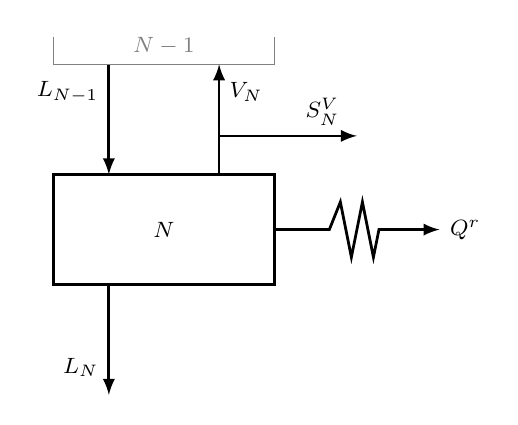
\begin{tikzpicture}[arrow/.style={line width=1pt,->,>=latex},scale=0.7]
	\draw [line width=1pt] (-2,1) rectangle (2,-1) node at (0,0) {\footnotesize $N$};
	\draw [arrow] (-1,3) -- (-1,1) node [pos=0.25, left] {\footnotesize $L_{N-1}$};
 	\draw [arrow] (1,1) -- (1,3) node [pos=0.75, right] {\footnotesize $V_{N}$};
 	\draw [arrow] (1,1.7) -- (3.5,1.7) node [pos=0.75, above] {\footnotesize $S^V_{N}$};
 	\draw [arrow] (-1,-1) -- (-1,-3) node [pos=0.75, left] {\footnotesize $L_{N}$};
	\draw [arrow] (2,0) -- (3,0) -- (3.2,0.5) -- (3.4,-0.5) -- (3.6,0.5) -- (3.8,-0.5) -- (3.9,0) -- (5,0,0) node [pos=1, right] {\footnotesize $Q^r$} ; 
    \draw [line width=0.5pt,gray] (-2,3.5) -- (-2,3) -- (2,3) node [pos=0.5, above] {\footnotesize $N-1$} -- (2,3.5) ;
\end{tikzpicture}

%\end{figure}
